\section{Zookeeper}

Zookeeper is essential in order to run Kafka. The role of Zookeeper in a Kafka cluster is configuration management. 
	
Zookeeper is a separate service with an exposed API, with clients in many languages. We use the clients to interact with the API. At a high-level Zookeeper stores configurations in a tree structure \cite{hunt2010zookeeper}. Each node in the tree is called a ZNode. Clients can connect to Zookeeper and watch for configuration changes. An example of a configuration change in Kafka may be that a new leader has been elected. All connected clients would receive this information and act accordingly. In figure \ref{fig:zookeeper-znodes} we see how Kafka can store information in znodes.

\begin{figure}[H]
  \centering
  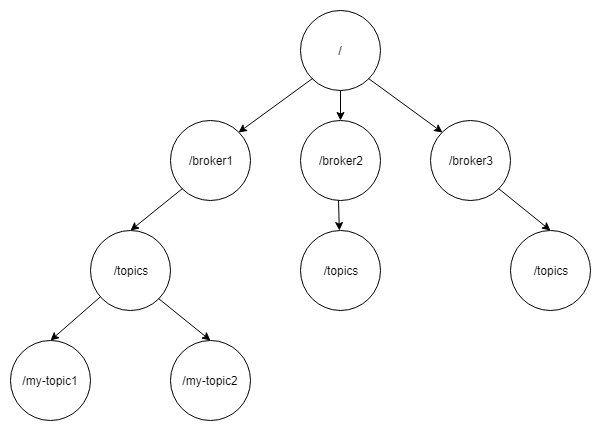
\includegraphics[scale=0.5,width=100mm]{./images/zookeeper-znodes.png}
  \caption{Zookeeper znode tree structure for Kafka}
  \label{fig:zookeeper-znodes}
\end{figure}

Zookeeper has a number of roles within a Kafka cluster. these are summarized below

\begin{itemize}
  \item Leader election when a broker fails.
  \item Maintains a list of all brokers that are currently alive and part of the cluster.
  \item Maintains a list of topics and how man partitions each one has, as well as the leader for each topic.
  \item A list of ACL's for each topic. The shows if we are allowed to read and write to a particular topic
\end{itemize}